% 若编译失败,且生成 .synctex(busy) 辅助文件,可能有两个原因:
% 1. 需要插入的图片不存在:Ctrl + F 搜索 'figure' 将这些代码注释/删除掉即可
% 2. 路径/文件名含中文或空格:更改路径/文件名即可

% --------------------- 文章宏包及相关设置 --------------------- %
% >> ------------------ 文章宏包及相关设置 ------------------ << %
% 设定文章类型与编码格式
\documentclass[UTF8]{article}		

% 物理实验报告所需的其它宏包
\usepackage{ulem}   % \uline 下划线支持
\usepackage{circuitikz} % 电路图 tikz 支持
\usepackage{pdfpages}   % 用于导入 pdf 文件
\usepackage{multirow}   % 用于表格合并单元格

% 本 .tex 专属的宏定义
    \def\V{\ \mathrm{V}}
    \def\uV{\ \mu\mathrm{V}}
    \def\mV{\ \mathrm{mV}}
    \def\K{\ \mathrm{K}}
    \def\kV{\ \mathrm{KV}}
    \def\KV{\ \mathrm{KV}}
    \def\MV{\ \mathrm{MV}}
    \def\uA{\ \mu\mathrm{A}}
    \def\mA{\ \mathrm{mA}}
    \def\A{\ \mathrm{A}}
    \def\kA{\ \mathrm{KA}}
    \def\KA{\ \mathrm{KA}}
    \def\MA{\ \mathrm{MA}}
    \def\O{\ \Omega}
    \def\mO{\ \Omega}
    \def\kO{\ \mathrm{K}\Omega}
    \def\KO{\ \mathrm{K}\Omega}
    \def\MO{\ \mathrm{M}\Omega}
    \def\Hz{\ \mathrm{Hz}}
    \def\uF{\ \mu\mathrm{F}}
    \def\mF{\ \mathrm{mF}}
    \def\F{\ \mathrm{F}}
    \def\Re{\mathrm{\,Re}\,}
    \def\Im{\mathrm{\,Im}\,}
    \def\sinc{\mathrm{\,sinc}\,}

% 自定义宏定义
    \def\N{\mathbb{N}}
    \def\F{\mathbb{F}}
    \def\Z{\mathbb{Z}}
    \def\Q{\mathbb{Q}}
    \def\R{\mathbb{R}}
    \def\C{\mathbb{C}}
    \def\T{\mathbb{T}}
    \def\S{\mathbb{S}}
    %\def\A{\mathbb{A}}
    \def\I{\mathscr{I}}
    \def\d{\mathrm{d}}
    \def\p{\partial}


% 导入基本宏包
    \usepackage[UTF8]{ctex}     % 设置文档为中文语言
    \usepackage{hyperref}  % 宏包:自动生成超链接 (此宏包与标题中的数学环境冲突)
    \hypersetup{
        colorlinks=true,    % false:边框链接 ; true:彩色链接
        citecolor={blue},    % 文献引用颜色
        linkcolor={blue},   % 目录 (我们在目录处单独设置),公式,图表,脚注等内部链接颜色
        urlcolor={orange},    % 网页 URL 链接颜色,包括 \href 中的 text
        % cyan 浅蓝色 
        % magenta 洋红色
        % yellow 黄色
        % black 黑色
        % white 白色
        % red 红色
        % green 绿色
        % blue 蓝色
        % gray 灰色
        % darkgray 深灰色
        % lightgray 浅灰色
        % brown 棕色
        % lime 石灰色
        % olive 橄榄色
        % orange 橙色
        % pink 粉红色
        % purple 紫色
        % teal 蓝绿色
        % violet 紫罗兰色
    }
    % \usepackage{docmute}    % 宏包:子文件导入时自动去除导言区,用于主/子文件的写作方式,\include{./51单片机笔记}即可。注:启用此宏包会导致.tex文件capacity受限。
    \usepackage{amsmath}    % 宏包:数学公式
    \usepackage{mathrsfs}   % 宏包:提供更多数学符号
    \usepackage{amssymb}    % 宏包:提供更多数学符号
    \usepackage{pifont}     % 宏包:提供了特殊符号和字体
    \usepackage{extarrows}  % 宏包:更多箭头符号 
    \usepackage{multicol}   % 宏包:支持多栏 

% 文章页面margin设置
    \usepackage[a4paper]{geometry}
        \geometry{top=0.75in}
        \geometry{bottom=0.75in}
        \geometry{left=0.75in}
        \geometry{right=0.75in}   % 设置上下左右页边距
        \geometry{marginparwidth=1.75cm}    % 设置边注距离(注释、标记等)

% 配置数学环境
    \usepackage{amsthm} % 宏包:数学环境配置
    % theorem-line 环境自定义
        \newtheoremstyle{MyLineTheoremStyle}% <name>
            {11pt}% <space above>
            {11pt}% <space below>
            {\kaishu}% <body font> 默认使用正文字体, \kaishu 为楷体
            {}% <indent amount>
            {\bfseries}% <theorem head font> 设置标题项为加粗
            {:\ \ }% <punctuation after theorem head>
            {.5em}% <space after theorem head>
            {\textbf{#1}\thmnumber{#2}\ \ (\,\textbf{#3}\,)}% 设置标题内容顺序
        \theoremstyle{MyLineTheoremStyle} % 应用自定义的定理样式
        \newtheorem{LineTheorem}{Theorem.\,}
    % theorem-block 环境自定义
        \newtheoremstyle{MyBlockTheoremStyle}% <name>
            {11pt}% <space above>
            {11pt}% <space below>
            {\kaishu}% <body font> 使用默认正文字体
            {}% <indent amount>
            {\bfseries}% <theorem head font> 设置标题项为加粗
            {:\\ \indent}% <punctuation after theorem head>
            {.5em}% <space after theorem head>
            {\textbf{#1}\thmnumber{#2}\ \ (\,\textbf{#3}\,)}% 设置标题内容顺序
        \theoremstyle{MyBlockTheoremStyle} % 应用自定义的定理样式
        \newtheorem{BlockTheorem}[LineTheorem]{Theorem.\,} % 使用 LineTheorem 的计数器
    % definition 环境自定义
        \newtheoremstyle{MySubsubsectionStyle}% <name>
            {11pt}% <space above>
            {11pt}% <space below>
            {}% <body font> 使用默认正文字体
            {}% <indent amount>
            {\bfseries}% <theorem head font> 设置标题项为加粗
            {:\\ \indent}% <punctuation after theorem head>
            {0pt}% <space after theorem head>
            {\textbf{#3}}% 设置标题内容顺序
        \theoremstyle{MySubsubsectionStyle} % 应用自定义的定理样式
        \newtheorem{definition}{}

%宏包:有色文本框(proof环境)及其设置
    \usepackage{xcolor}    %设置插入的文本框颜色
    \usepackage[strict]{changepage}     % 提供一个 adjustwidth 环境
    \usepackage{framed}     % 实现方框效果
        \definecolor{graybox_color}{rgb}{0.95,0.95,0.96} % 文本框颜色。修改此行中的 rgb 数值即可改变方框纹颜色,具体颜色的rgb数值可以在网站https://colordrop.io/ 中获得。(截止目前的尝试还没有成功过,感觉单位不一样)(找到喜欢的颜色,点击下方的小眼睛,找到rgb值,复制修改即可)
        \newenvironment{graybox}{%
        \def\FrameCommand{%
        \hspace{1pt}%
        {\color{gray}\vrule width 2pt}%
        {\color{graybox_color}\vrule width 4pt}%
        \colorbox{graybox_color}%
        }%
        \MakeFramed{\advance\hsize-\width\FrameRestore}%
        \noindent\hspace{-4.55pt}% disable indenting first paragraph
        \begin{adjustwidth}{}{7pt}%
        \vspace{2pt}\vspace{2pt}%
        }
        {%
        \vspace{2pt}\end{adjustwidth}\endMakeFramed%
        }

% 外源代码插入设置
    % matlab 代码插入设置
    \usepackage{matlab-prettifier}
        \lstset{style=Matlab-editor}    % 继承 matlab 代码高亮 , 此行不能删去
    \usepackage[most]{tcolorbox} % 引入tcolorbox包 
    \usepackage{listings} % 引入listings包
        \tcbuselibrary{listings, skins, breakable}
        \newfontfamily\codefont{Consolas} % 定义需要的 codefont 字体
        \lstdefinestyle{MatlabStyle_inc}{   % 插入代码的样式
            language=Matlab,
            basicstyle=\footnotesize\ttfamily\codefont,    % ttfamily 确保等宽 
            breakatwhitespace=false,
            breaklines=true,
            captionpos=b,
            keepspaces=true,
            numbers=left,
            numbersep=15pt,
            showspaces=false,
            showstringspaces=false,
            showtabs=false,
            tabsize=2,
            xleftmargin=15pt,   % 左边距
            %frame=single, % single 为包围式单线框
            frame=shadowbox,    % shadowbox 为带阴影包围式单线框效果
            %escapeinside=``,   % 允许在代码块中使用 LaTeX 命令 (此行无用)
            %frameround=tttt,    % tttt 表示四个角都是圆角
            framextopmargin=0pt,    % 边框上边距
            framexbottommargin=0pt, % 边框下边距
            framexleftmargin=5pt,   % 边框左边距
            framexrightmargin=5pt,  % 边框右边距
            rulesepcolor=\color{red!20!green!20!blue!20}, % 阴影框颜色设置
            %backgroundcolor=\color{blue!10}, % 背景颜色
        }
        \lstdefinestyle{MatlabStyle_src}{   % 插入代码的样式
            language=Matlab,
            basicstyle=\small\ttfamily\codefont,    % ttfamily 确保等宽 
            breakatwhitespace=false,
            breaklines=true,
            captionpos=b,
            keepspaces=true,
            numbers=left,
            numbersep=15pt,
            showspaces=false,
            showstringspaces=false,
            showtabs=false,
            tabsize=2,
        }
        \newtcblisting{matlablisting}{
            %arc=2pt,        % 圆角半径
            % 调整代码在 listing 中的位置以和引入文件时的格式相同
            top=0pt,
            bottom=0pt,
            left=-5pt,
            right=-5pt,
            listing only,   % 此句不能删去
            listing style=MatlabStyle_src,
            breakable,
            colback=white,   % 选一个合适的颜色
            colframe=black!0,   % 感叹号后跟不透明度 (为 0 时完全透明)
        }
        \lstset{
            style=MatlabStyle_inc,
        }

% table 支持
    \usepackage{booktabs}   % 宏包:三线表
    \usepackage{tabularray} % 宏包:表格排版
    \usepackage{longtable}  % 宏包:长表格

% figure 设置
    \usepackage{graphicx}  % 支持 jpg, png, eps, pdf 图片 
    \usepackage{svg}       % 支持 svg 图片
        \svgsetup{
            % 指向 inkscape.exe 的路径
            inkscapeexe = C:/aa_MySame/inkscape/bin/inkscape.exe, 
            % 一定程度上修复导入后图片文字溢出几何图形的问题
            inkscapelatex = false                 
        }
    \usepackage{subcaption} % 用于子图和小图注  

% 图表进阶设置
    \usepackage{caption}    % 图注、表注
        \captionsetup[figure]{name=图}  
        \captionsetup[table]{name=表}
        \captionsetup{
            labelfont=bf, % 设置标签为粗体
            textfont=bf,  % 设置文本为粗体
            font=small  
        }
    \usepackage{float}     % 图表位置浮动设置 
    \usepackage{etoolbox} % 用于保证图注表注的数学字符为粗体
        \AtBeginEnvironment{figure}{\boldmath} % 图注中的数学字符为粗体
        \AtBeginEnvironment{table}{\boldmath}  % 表注中的数学字符为粗体
        \AtBeginEnvironment{tabular}{\unboldmath}   % 保证表格中的数学字符不受额外影响

% 圆圈序号自定义
    \newcommand*\circled[1]{\tikz[baseline=(char.base)]{\node[shape=circle,draw,inner sep=0.8pt, line width = 0.03em] (char) {\bfseries #1};}}   % TikZ solution

% 列表设置
    \usepackage{enumitem}   % 宏包:列表环境设置
        \setlist[enumerate]{
            label=(\arabic*) ,   % 设置序号样式为加粗的 (1) (2) (3)
            ref=\arabic*, % 如果需要引用列表项,这将决定引用格式(这里仍然使用数字)
            itemsep=0pt, parsep=0pt, topsep=0pt, partopsep=0pt, leftmargin=3.5em} 
        \setlist[itemize]{itemsep=0pt, parsep=0pt, topsep=0pt, partopsep=0pt, leftmargin=3.5em}
        \newlist{circledenum}{enumerate}{1} % 创建一个新的枚举环境  
        \setlist[circledenum,1]{  
            label=\protect\circled{\arabic*}, % 使用 \arabic* 来获取当前枚举计数器的值,并用 \circled 包装它  
            ref=\arabic*, % 如果需要引用列表项,这将决定引用格式(这里仍然使用数字)
            itemsep=0pt, parsep=0pt, topsep=0pt, partopsep=0pt, leftmargin=3.5em
        }  

% 其它设置
    % 脚注设置
        \renewcommand\thefootnote{\ding{\numexpr171+\value{footnote}}}
    % 参考文献引用设置
        \bibliographystyle{unsrt}   % 设置参考文献引用格式为unsrt
        \newcommand{\upcite}[1]{\textsuperscript{\cite{#1}}}     % 自定义上角标式引用
    % 文章序言设置
        \newcommand{\cnabstractname}{序言}
        \newenvironment{cnabstract}{%
            \par\Large
            \noindent\mbox{}\hfill{\bfseries \cnabstractname}\hfill\mbox{}\par
            \vskip 2.5ex
            }{\par\vskip 2.5ex}

% 文章默认字体设置
    \usepackage{fontspec}   % 宏包:字体设置
        \setmainfont{SimSun}    % 设置中文字体为宋体字体
        \setCJKmainfont[AutoFakeBold=3]{SimSun} % 设置加粗字体为 SimSun 族,AutoFakeBold 可以调整字体粗细
        \setmainfont{Times New Roman} % 设置英文字体为Times New Roman

% 各级标题自定义设置
    \usepackage{titlesec}   
        % section标题自定义设置 
        \titleformat{\section}[hang]{\normalfont\Large\bfseries\boldmath}{\thesection}{8pt}{}
        % subsection 标题自定义设置
        \titleformat{\subsection}[hang]{\normalfont\large\bfseries\boldmath}{\thesubsection}{8pt}{}
        \titlespacing*{\subsection}{0pt}{10pt}{6pt} % 控制上下间距


% --------------------- 文章宏包及相关设置 --------------------- %
% >> ------------------ 文章宏包及相关设置 ------------------ << %


% ------------------------ 文章信息区 ------------------------ %
% ------------------------ 文章信息区 ------------------------ %
% 页眉页脚设置
\usepackage{fancyhdr}   %宏包:页眉页脚设置
    \pagestyle{fancy}
    \fancyhf{}
    \cfoot{\thepage}
    \renewcommand\headrulewidth{1pt}
    \renewcommand\footrulewidth{0pt}
    \rhead{\bfseries \large {\color{red} 分组序号: 2-05}}    
    \chead{《基础物理实验》预习报告,\ 丁毅,\ 2023K8009908031}
    \lhead{\small Ex.01 杨氏模量 (2024.11.12)}

% 开始编辑文章

\begin{document}
\begin{center}\large
    \vspace*{-0.8cm}
    \noindent{\huge\bfseries《\ \ 基\ \ 础\ \ 物\ \ 理\ \ 实\ \ 验\ \ \ 》\ \ 预\ \ 习\ \ 报\ \ 告 }
    \\\vspace{0.1cm}
    \noindent{
    {\bfseries 
    实验名称:\uline{\hspace{1.3cm} 杨氏模量与微小量测量 \hspace{1.3cm}}
    }\hspace{0.4cm}
    指导教师:\uline{\hspace{2.6cm} \ \ \hspace{2.6cm}}
    }
    \\\vspace{0.1cm}
    \noindent
    {
    姓名:\uline{\,\,\,丁毅\,\,\,}\hspace{0.2cm}
    学号:\uline{\,\,\,{ 2023K8009908031}\,\,\,}\hspace{0.2cm}
    班级/专业:\uline{\,\,\,{2308/电子信息}\,\,\,}\hspace{0.2cm}
    分组序号:\uline{\,\,\,{2-05}\,\,\,}
    }
    \\\vspace{0.1cm}
    \noindent{
    实验日期:\uline{\,\,{ 2024.11.12}\,\,}\hspace{0.2cm}
    实验地点:\uline{\,\,\,教学楼{ 710}\,\,\,}\hspace{0.2cm}
    是否调课/补课:\uline{\hspace{0.26cm}否 \hspace{0.26cm}}\hspace{0.2cm}
    成绩:\uline{\hspace{2cm}}
    }
\end{center}
\vspace{-0.4cm}
\noindent\rule{\textwidth}{0.075em}   % 分割线
\vspace{-1.0cm}

% 目录
\setcounter{tocdepth}{2}  % 目录深度为 2(不显示 subsubsection)
\noindent\tableofcontents\thispagestyle{fancy}   % 显示页码、页眉等
\newpage
\rhead{\bfseries\small 分组序号: 2-05}
% ------------------------ 文章信息区 ------------------------ %
% ------------------------ 文章信息区 ------------------------ %


%% 下面是正文内容


\section{实验目的}
\begin{enumerate}
\item 理解测量杨氏模量的静态法和动态法的相关原理,尤其是前者各种方法对测量微小位移的优缺点;
\item 熟悉霍尔位置传感器的特性,理解传感器相关曲线的意义;
\item 了解光杠杆法的原理和适用范围;
\item 学会对一些实验器材的规范调节,比如读数望远镜、读数显微镜等;
\item 学习用逐差法、作图法和最小二乘法处理数据;
\item 学会计算各物理量的不确定度,并用不确定度正确表达实验结果。
\end{enumerate}


\section{拉伸法}
\subsection{实验仪器与用具}

CCD 杨氏弹性模量测量仪(LB-YM1 型、YMC-2 型)、螺旋测微器、钢卷尺等。
\begin{figure}[H]\centering
    \includegraphics[width=0.4\columnwidth]{assets/0/da2dd09fb93428ae0fb1bc23c8c81af2.png}
    \caption{LB-YM1 型实验装置}
\end{figure}

其主要技术指标如下:采用
分划板(刻度范围 4mm,分度值 0.05mm,设有限位槽,可防止来回摆动,
采用LED 照明)+
CCD测量显微镜系统(放大倍率60倍,内含电子刻度线,可二维调节,
可卸下用于其他微位移测量场合)+
彩色液晶监视器方案.

\subsection{实验原理}
物体在外力作用下都会发生形变。当形变在一定限度内,撤走外力能恢复原状的形变称为弹性形变。
反之撤走外力之后仍有剩余形变,称为塑性形变。发生弹性形变时,弹性模量便是反应材料形变与内应力关系的基本物理量。

设柱状物体的长度为$L$,截面积为$S$,沿长度方向受外力$F$作用后伸长(或缩短)量为$\Delta L$,单位横截面积上垂
直作用力$F/S$称为正应力,物体的相对伸长$\Delta L/L$称为线应变。胡克定律告诉我们:
\begin{equation}
   F/S=Y\frac{\Delta L}{L} 
\end{equation}
其中$Y$便称为杨氏模量,本实验中我们将以显微镜和CCD成像系统进行对$\Delta L$的测量,并通过砝码测量外力,通过钢卷尺测量金属丝长度,
通过螺旋测微器测量金属丝直径,从而将知道有公式:
\begin{equation}
    Y=\frac{4FL}{\pi d^2\Delta L}
\end{equation}

\subsection{实验注意事项}
\begin{enumerate}
\item 需保证分划板卡在下衡梁的槽内,避免其在拉直过程中旋转。

\item 轻轻加减砝码,防止使砝码盘产生微小振动而造成读数起伏较大,或者钼丝突然受力而断裂。

\item 多次测量数据并求平均,包括叉丝读数,金属丝长度和直径等,读数需等刻度值稳定后。

\item CCD器件不可正对太阳、激光或其他强光源。注意保护镜头,防
潮、防尘、防污染。

\item 金属丝必须保持铅直形态。测直径时要特别谨慎,避免由于扭转、拉扯、牵挂导致细丝
折弯变形。

\item 做完实验后归类收纳好各种实验器材。
\end{enumerate}


\subsection{实验步骤}
\begin{enumerate}
\item 仪器调整——例如工作台调平、金属丝安装、夹头调整以及其他实验设备的连接。
打开CCD并进行显微镜的调节,利用磁力滑座与三维调整台在屏幕上先调出数字分划板及十字叉丝,接着
进行显微镜的对焦与对准十字叉丝(使之尽量与读数轴平行)。

\item 测量与数据记录——测量钼丝的几何尺寸(有效长度、直径等)。
随后将砝码依次放置并读取数值(等待CCD成像稳定后,可能还需要重新对焦),
再依次取下并读取数值.加减砝码时,
动作要轻,防止因增减砝码时使砝码盘产生微小振动而造成读数起伏较大。
而且不要晃桌子,以免晃动后分划板倾斜造成读数的较大误差。

\item 实验结束后归类收纳好各种实验器材.
\end{enumerate}


\section{霍尔法(弯曲法)}
\subsection{实验仪器与用具}

杭州大华DHY-1A霍尔位置传感器法杨氏模量测定仪:
包括底座固定箱、读数显微镜及调节机构、
SS495A型集成霍尔位置传感器(灵敏度大于250$\rm mV/mm$,线性范围为0-2mm)、
测试仪、磁体、支架、加力机构等。
样品为黄铜条、铸铁条。
测试仪由霍尔电压测量系统和电子称加力系统构成,
霍尔电压测试分为两个量程,
带调零功能;电子称加力系统测量范围$0\sim199.9\,\,{\rm g}$,连续可调,三位半数显。

\begin{figure}[H]\centering
\begin{subfigure}[b]{0.4\columnwidth}\centering
    \includegraphics[height=150pt]{assets/0/image (19).png}
    \caption{实验装置图}
\end{subfigure}\hfill
\begin{subfigure}[b]{0.6\columnwidth}\centering
    \includegraphics[height=150pt]{assets/0/image (20).png}
    \caption{实验装置图}
\end{subfigure}
\caption{霍尔法测量杨氏模量}
\end{figure}

读数显微镜的技术指标:型号JC-10型,目镜放大率10倍,目镜测微鼓轮最小分度值为0.01 mm,物镜放大率为2倍,测量范围为0-6mm,实际读书最小分辨率为0.005mm;

霍尔电压表的技术指标:量程0-199.9mV,分辨率为0.1mV

\subsection{实验原理}


霍尔元件在磁感应强度为$B$的磁场和电流$I$的作用下,产生霍尔电势差\begin{displaymath}U_H=K\cdot I\cdot B\end{displaymath}而在保持电流不变的情况下,在一个具均匀梯度的磁场下运动时,
输出的霍尔电势差的变化量为\begin{displaymath}\Delta U_H=K\cdot I\cdot \frac{\mathrm{d}B}{\mathrm{d}Z}\Delta Z\end{displaymath}其中上式的$\Delta Z$是位移量,
故而上式表明,
当磁场的梯度变化为恒定时,$\Delta U_H$与$\Delta Z$成正比,而这正是我们进行测量杨氏模量的理论基础:
霍尔电势差和位移量之间存在一一对应的关系,
所以在当位移量不太大的时候,
该一一对应的关系具有良好的线性。


如下图所示,设金属篇在刀口间的长度为$ d $,金属片的厚度为$ a $,宽度为$ b $。

\begin{figure}[H]\centering
    \resizebox{!}{150pt}{
        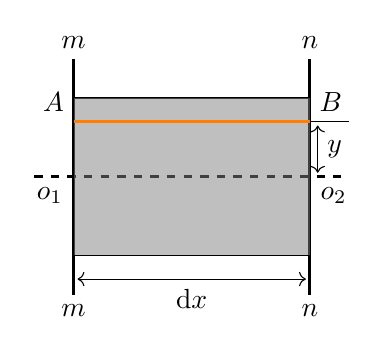
\begin{tikzpicture}
            \draw[dashed,very thick] (-2,0)--(-1.5,0) node[below left]{$ o_1 $}--(1.5,0) node[below right]{$ o_2 $}--(2,0);
            \draw[very thick] (-1.5,-1.5)--(-1.5,1.5);
            \draw[very thick] (1.5,-1.5)--(1.5,1.5);
            \draw (-1.5,-1)--(1.5,-1);
            \draw (-1.5,1)--(1.5,1);
            \fill[gray,fill opacity=0.5] (-1.5,-1) rectangle (1.5,1);
            \draw[<->] (-1.45,-1.3)--(1.45,-1.3);
            \node[below] at(0,-1.3) {$ \mathrm{d} x $};
            \node[below] at(-1.5,-1.5) {$ m $};
            \node[below] at(1.5,-1.5) {$ n $};
            \node[above] at(-1.5,1.5) {$ m $};
            \node[above] at(1.5,1.5) {$ n $};
            \draw[very thick,orange] (-1.5,0.7)--(1.5,0.7);
            \node[above left] at(-1.5,0.7) {$ A $};
            \node[above right] at(1.5,0.7) {$ B $};
            \draw (1.5,0.7)--(2,0.7);
            \draw[<->] (1.6,0.05)--(1.6,0.65);
            \node[right] at(1.6,0.35) {$ y $};
        \end{tikzpicture}
    }\hspace*{1cm}
    \resizebox{!}{150pt}{
        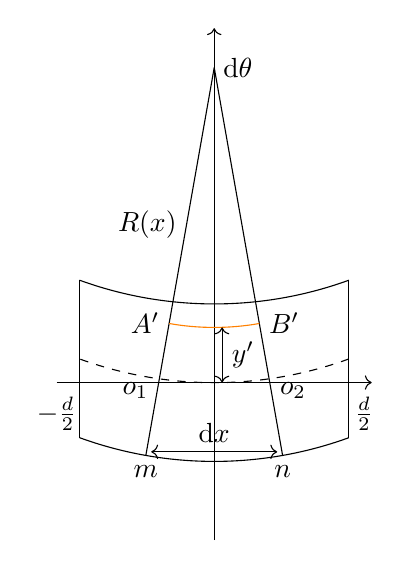
\begin{tikzpicture}
            \draw (1.71,0.3) arc (290:250:5);
            \draw (1.71,2.3) arc (290:250:5);
            %\draw (0,5)--(1,5);
            \draw (1.71,0.3)--(1.71,2.3);
            \draw (-1.71,0.3)--(-1.71,2.3);
            \draw (0.8682,0.0760)node[below]{$ n $} -- (0,5);
            \draw (-0.8682,0.0760)node[below]{$ m $} -- (0,5);
            \draw[->] (0,-1)--(0,5.5);
            \draw[->] (-2,1)--(2,1);
            \draw[dashed] (1.71,1.3) arc (290:250:5);
            \draw[<->] (-0.8,0.12)--node[above]{$ \mathrm{d} x $} (0.8,0.12);
            \node at(1.9,0.6) {$ \frac d2 $};
            \node at(-2,0.6) {$ -\frac d2 $};
            \node at(-1,0.9) {$ o_1 $};
            \node at(1,0.9) {$ o_2 $};
            \node at(-0.85,3) {$ R(x) $};
            \node at(0.3,5) {$ \mathrm{d}\theta $};
            \draw[orange] (0.573,1.7501) arc (280:260:3.3);
            \node[left] at(-0.573,1.7501) {$ A' $};
            \node[right] at(0.573,1.7501) {$ B' $};
            \draw[<->] (0.1,1)--node[right]{$ y' $} (0.1,1.7);
        \end{tikzpicture}
    }
    \caption{弯曲法测杨氏模量原理示意图}
\end{figure}



$ o_1o_2 $所在平面为中性面,既不拉伸也不压缩,$ AB $为距中性面距离$ y $处的平面。变形前有$ o_1o_2=AB=\mathrm{d} x $,变形后则为$ o_1o_2=\mathrm{d} x=R(x)\mathrm{d}\theta,\;A'B'=(R(x)-y)\mathrm{d}\theta $.

那么$ AB $面的应变为
\begin{equation}
\varepsilon=\frac{A'B'-AB}{AB}=\frac{(R(x)-y)\mathrm{d}\theta-\mathrm{d} x}{\mathrm{d} x}=\frac{(R(x)-y)\dfrac{\mathrm{d} x}{R(x)}-\mathrm{d} x}{\mathrm{d} x}=-\frac{y}{R(x)}
\end{equation}
根据胡克定律$ \frac{\mathrm{d} F}{\mathrm{d} S}=Y\varepsilon=-Y\frac{y}{R(x)} $且$ \mathrm{d} S=b\mathrm{d} y $,因此有
\begin{equation}
\mathrm{d} F(x)=-\frac{Y\mathrm{d} y}{R(x)}\mathrm{d} y
\end{equation}
对中性面的转矩为
\begin{equation}\label{2-1}
    \mathrm{d}\mu(x)=|\mathrm{d} F(x)|y=\frac{Yb}{R(x)}y^2\mathrm{d} y
\end{equation}
积分可得
\begin{equation}
\mu(x)=\int_{-a/2}^{a/2}\frac{Yb}{R(x)}y^2\mathrm{d} y=\frac{Yba^3}{12R(x)}
\end{equation}
对梁上各点有$ \frac{1}{R(x)}=\frac{y''(x)}{[1+y'(x)]^{3/2}} $,由于梁的弯曲很小,$ y'(x)=0 $,所以
\begin{equation}\label{2-2}
    R(x)=\frac{1}{y''(x)}
\end{equation}
在平衡时,梁在$ x $处的转矩应与梁右端支撑力$ \frac{Mg}{2} $对$ x $处的力矩平衡,因此有
\begin{equation}\label{2-3}
    \mu(x)=\frac{Mg}{2}\left(\frac d2-x\right)
\end{equation}
由(\ref{2-1}),(\ref{2-2}),(\ref{2-3})可得
\begin{equation}
y''(x)=\frac{6Mg}{Yba^3}\left(\frac d2-x\right)
\end{equation}
代入边界条件$ y(0)=0,\;y'(0)=0 $可求得
\begin{equation}
y(x)=\frac{3Mg}{Yba^3}\left(\frac d2x^2-\frac13x^3\right)
\end{equation}
在中点$ x=\frac d2 $处,有
\begin{equation}
\Delta z=y\left(\frac d2\right)=\frac{Mgd^3}{4Yba^3}
\end{equation}
所以杨氏模量为
\begin{equation}\label{2}
    Y=\frac{d^3Mg}{4a^3b\Delta Z}
\end{equation}
其中$ d $为两刀口间的距离,$ M $为所加拉力对应的质量,$ a $为梁的厚度,$ b $为梁的宽度,$ \Delta Z $为梁中心由于外力作用而下降的距离,$ g $为重力加速度。


\subsection{实验注意事项}
\begin{enumerate}
\item 用千分尺待测样品厚度必须不同位置多点测量取平均值,并且测量黄铜时,用力需适度。

\item 用读数显微镜测量铜刀口基线位置时,刀口不能晃动。

\item 调整霍尔传感器水平,并对各种元件作位置检查和数字归零处理,

\item 实验结束后,关闭电源,整理实验桌面,实验器材放置于实验初始位置。
\end{enumerate}



\subsection{实验步骤}

\begin{enumerate}
\item 调平——首先用水平泡观察平台是否处于水平位置, 若偏离时调节下方水平调节机脚. 

\item 实验装置的调整——大致安装好实验仪器的相对位置,通过磁体调节结构上下移动磁铁使集成霍尔位置传感器探测元件处于磁铁中间的位置(此处磁场可视为均匀).
调节好后固定,最后在拉力绳不受力的情况下将电子称传感器加力系统进行调零.


\item 调节读数显微镜——轻微转动或调整使眼睛观察到清晰的十字线及分划板刻度线和数字. 然后移动读数显微镜前后距离, 直到
清晰看到铜刀口上的黑色基线. 使用适当的力锁紧加力旋钮旁边的锁紧螺钉, 转动读数显微镜读数鼓轮使
铜刀口上的基线与读数显微镜内十字刻度线吻合.

\item 读取数据——通过加力调节旋钮逐次增加拉力 (每次增加10g) , 相应从读数显微镜上读出梁的弯曲位移$\Delta Z_i$及霍尔数
字电压表相应的读数值$U_i$(单位 mV) . 以便计算杨氏模量和对霍尔位置传感器进行定标.

\item 测量几何尺寸——实验完毕松开加力旋钮旁边的锁紧螺钉, 松开加力旋钮, 取下样品.接着多次测量并记录试样在两刀口间的长度 d、不同位置黄铜宽度 b 以及黄铜厚度 a.

\item 整理实验桌面——关闭电源, 整理实验桌面, 实验器材放置于实验初始位置.
\end{enumerate}



\section{动态悬挂法}
\subsection{实验仪器与用具}
DHY-2A 型动态杨氏模量测试台、DH0803 振动力学通用信号源,
通用示波器、
测试棒(铜、不锈钢)、悬线、专用连接导线、天平、游标卡尺、螺旋测微计等。

\begin{figure}[H]\centering
    \includegraphics[width=0.75\columnwidth]{assets/0/a36e12208fcd72455f93e4b950ef3249.png}
    \caption{DHY-2A 型动态杨氏模量测试装置}
\end{figure}


\subsection{实验原理}

先令$y$为棒振动的位移,$Y$为棒振动的杨氏模量,$S$为棒的横截面积,$J$为棒的转动惯量,$\rho$为棒密度,$x$为位置坐标,$t$为时间变量
通过分离变数法(即令$y(x,t)=X(x),T(t)$)可解得
\begin{equation}
    y(x,t)=\left(A_1{\rm ch}K_x+A_2{\rm sh}K_x+B_1\cos K_x+B_2\sin K_x \right)\cos (\omega t+\varphi)
\end{equation}
其中$\omega=\left(K^4YJ/\rho S\right)^{1/2}$称为频率公式,$K$为常数,$A_1,A_2,B_1,B_2,\varphi$为待定常数,可由边界和初始条件确定。

对于长为$L$,两端自由的棒,当悬线悬挂于棒的节点附近时,其边界条件为:
自由端横向作用力$F$为零,弯矩$M$亦为零:
\begin{equation}
   F=-\frac{\partial M}{\partial x} =0\qquad 
   M=EJ\frac{\partial^2y}{\partial x^2}=0
\end{equation}

将边界条件带入通解$y=(x,t)$中可的超越方程$\cos KL\cdot {\rm ch}KL=1$.
其第一个根为$0$,对应于静态值,第二个根$K_1L\approx 4.7300$,此时的共振频率称为基频(或固有频率)$\omega_1=2\pi f_1$。
对于直径为$d$,长为$L$,质量为$m$的圆形棒,可知在此频率下共振时,其杨氏模量:
\begin{equation}
   Y=1.6067\frac{L^3mf_1^2}{d^4} 
\end{equation}





测试棒在作基频振动时存在两个节点,它们的位置距离端面$0.224L $(距离另一端面为$0.776L$)
处,理论上,悬挂点应取在节点处测试棒难于被激振和拾振,为此可在节点两旁选不同点对称悬挂,用外推法找出节点处的共振频率。


\subsection{实验注意事项}

\begin{enumerate}
\item 本实验中只能测出的共振频率。但由于二者相差很小,故固有频率可用共振频率代替。

\item 安装测试棒时,应先移动支架到既定位置,再悬挂,需保证横向水平,悬线与测试棒轴向垂直。

\item 在示波器显示出现共振现象之后,需十分缓慢地微调频率调节细调旋钮,使波形振幅达到极大值。

\item 因为设备尺寸原因,部分设备在$0.0365L$、$ 0.9635L$处悬线不能竖直,此时该点要丢弃不测。

\item 每次测量时都用这种方法判别其是否为基频:沿测试棒长度的方向轻触棒的不同部位,观察示波器,在波节处波幅不变化,
而在波腹处,波幅会变小,并发现测试棒上有两个波节。

\end{enumerate}

\subsection{实验步骤}
\begin{enumerate}
\item 正确连接装置。

\item 测量共振频率:待测试棒稳定后,调节信号源发出信号的频率和幅度(先粗调再微调,可按照位数从高到低开始调节),寻找测试棒的共振频率:表示为示波器上正弦波幅度最大值(实际过程中变化可能有延迟,需要等待波形稳定后进行判断),并进行数据的记录,重复上述操作。

\item 实验结束后归纳并整理好实验台面。

\end{enumerate}

\section{光杠杆法}
\subsection{实验仪器与用具}
光杠杆测量系统(光杠杆反射镜、倾角调节架、标尺、
望远镜及调节反射镜等)、游标卡尺、螺旋测微器等。

\subsection{实验原理}

实际上就是采取了一种“放大”的思路,如下图所示:
\begin{figure}[H]
    \centering
    %\includegraphics[height=5cm]{光杠杆法.png}
    \caption{光杠杆法测量原理示意图}
\end{figure}
当钢丝的长度发生变化时,光杠杆的镜面必然不再竖直,有一角度变化。经过光路放大之后,便得到可以显著测量到的量:
\begin{equation}
    \Delta L=b\tan \theta\quad 2\theta \approx \frac{C/2}{H}
    \quad E=\frac{16FLH}{\pi D^2bC}
\end{equation}
这就得到了我们在本实验中需要依照的公式,其中用到了小角近似。


\subsection{实验注意事项}
\begin{enumerate}
\item 本实验由此需要细致调节:先目测调整之后,在通过调节望远镜的目镜旋轮,使“十”字清晰成像,随后细调光路至水平。
\item 注意测量中的误差记录与分析,并多次测量求平均以尽可能达到最佳的实验精度。

\end{enumerate}


\section{数据处理:不确定度与误差传递}

本次实验的一大重点就是理解并掌握数据的有效数字及不确定度的计算与合成,
故专门开一小节讨论。

\subsection*{6.1 \ 不确定度 $\Delta N$}

用以表示测量值不确定的程度,
反应数据的可信度,是测量结果质量的指标。测量结果一般表示为$Y=N+\Delta N$的形式,并且将$\Delta N/N$称为数据的相对不确定度。

\subsection*{6.2 \ 两类不确定度(A 类与 B 类)}


A类不确定度$u_A(x)$:即用以表示同样环境条件下多次
估读测量造成的不确定度(也称为标准偏差),表示为:
\begin{equation}
   u_A(x)=\sqrt{\frac{\sum_{i=1}^n(x_i-\overline x)^2}{n(n-1)}}\qquad \text{其中}\overline x=\frac{\sum_{i=1}^nx_i}{n} 
\end{equation}

B类不确定度$u_B(x)$:又分为单次测量时估读造成的不确定度$u_{B1}(x)$与仪器不确定度$u_{B2}(x)$,表示为:
\begin{equation}
   u_{B1}(x)=d,\frac{d}{10},\frac{d}{5}\qquad u_{B2}(x)=\frac{e}{\sqrt 3} 
\end{equation}
本次实验中取$u_{B1}(x)=\frac{d}{10}$,其中$d$为仪器最小分度值,$e$为仪器所示的最大误差,也称为允差。

\subsection*{6.3 \ 不确定度的合成}

多次测量时:
\begin{equation}
   u(x)=\sqrt{u_A^2(x)+u^2_{B2}(x)} 
\end{equation}
单次测量时:
\begin{equation}
    u(x)=\sqrt{u_{B1}^2(x)+u^2_{B2}(x)} 
\end{equation}
特别地,在长度测量中,因为读数时两个位置之差,故
\begin{equation}
    u(x)=\sqrt{u_{B1}^2(x)+u_{B1}^2(x)+u^2_{B2}(x)} =\sqrt{2u_{B1}^2(x)+u^2_{B2}(x)} 
\end{equation}


\section{思考题}

\section{实验总结与心得体会}







































%\newpage
%\section*{附录 A\hspace*{20pt} 手写预习报告}
%\addcontentsline{toc}{section}{附录 A\hspace*{6pt} 手写预习报告} 
\thispagestyle{fancy} 

%\begin{figure}[H]\centering
    %\includepdf[pages=1, width=480pt]{pdf/预习报告-2-05组-丁毅-傅里叶光学-2024.11.5-张秋琳.pdf}
%\end{figure}
%\includepdf[pages={2}]{pdf/预习报告-2-05组-丁毅-傅里叶光学-2024.11.5-张秋琳.pdf}

%\section*{附录 B\hspace*{20pt} Matlab 源码}
%\addcontentsline{toc}{section}{附录 B\hspace*{6pt} Matlab 源码} 
\thispagestyle{fancy} 
%\lstinputlisting{d:/a_RemoteRepo/GH.MatlabCodes/本科课程代码/基础物理实验/Ex_10_mfile.m}



\end{document}

% VScode 常用快捷键:

% F2:                       变量重命名
% Ctrl + Enter:             行中换行
% Alt + up/down:            上下移行
% 鼠标中键 + 移动:           快速多光标
% Shift + Alt + up/down:    上下复制
% Ctrl + left/right:        左右跳单词
% Ctrl + Backspace/Delete:  左右删单词    
% Shift + Delete:           删除此行
% Ctrl + J:                 打开 VScode 下栏(输出栏)
% Ctrl + B:                 打开 VScode 左栏(目录栏)
% Ctrl + `:                 打开 VScode 终端栏
% Ctrl + 0:                 定位文件
% Ctrl + Tab:               切换已打开的文件(切标签)
% Ctrl + Shift + P:         打开全局命令(设置)

% Latex 常用快捷键:

% Ctrl + Alt + J:           由代码定位到PDF


